% Source: Weinberg GR, physical PDF pp. 556--573
%         (printed pp. 528--545; boundary pages are partial).
% Coverage: Section 15.6, Thermal History of the Early Universe;
%           equations (15.6.1)--(15.6.70), including all unnumbered displays.
% Figures/tables/footnotes: Figure 15.5; Table 15.4; reference notes
%           87--98 and 173.
% Status: source-reviewed and compile-clean; visually proofed.
% Uncertainties: none.
% MODERNIZATION: the source cosmological scale factor is written a(t), with
% a_0=a(t_0), while the black-body radiation constant is a_{\mathrm{rad}}.
% The standard spelling “deceleration” is used. No signature-dependent
% four-vector or curvature expression occurs in this section.
% The source's unrelated beta-decay normalization a is denoted \alpha to
% avoid a second collision with the scale factor.
% LITERAL-OPERATOR AUDIT: every leading sign and continuation operator in
% equations (15.6.1)--(15.6.70), including the entropy, energy-density, and
% degenerate-neutrino integrals, was checked against physical pp. 556--573.

\subsection{Thermal History of the Early Universe}\label{sec:15.6}

The energy density of the present \(2.7^\circ\mathrm K\) microwave background
is
\begin{equation}
  \rho_{\gamma0}
  =
  a_{\mathrm{rad}}T_{\gamma0}^4
  =
  3.97\times10^{-13}\,\mathrm{erg/cm^3}
  =
  4.40\times10^{-34}\,\mathrm{g/cm^3}.
  \tag{15.6.1}\label{eq:15.6.1}
\end{equation}
As already remarked in Section~\ref{sec:15.2}, this is considerably less than
the present nucleonic rest-mass density, so that we presently are in a
matter-dominated era, which has lasted throughout most of the history of the
universe. This era was discussed in detail in Section~\ref{sec:15.3}.

We now turn our attention back to an earlier period, when radiation and
relativistic particles were more important than ordinary matter. In order to
avoid losing the thread of our story in the details of our calculations, it may
help to outline first what is now commonly pictured to be the early history of
the universe, and then go into the detailed calculations that support this
picture. The outline of universal history is currently believed to be something
as follows (see Figure~\ref{fig:15.5}).

\emph{(A)} At very early times, when the temperature \(T\) was above
\(10^{12\,\circ}\mathrm K\), the universe contained a great variety of
particles in thermal equilibrium, including photons, leptons, mesons, and
nucleons and their antiparticles. The strong interactions among mesons and
nucleons make this era very difficult to study; it will be discussed briefly
in Section~\ref{sec:15.11}.

\emph{(B)} At the time when \(T\simeq10^{12\,\circ}\mathrm K\), the universe
contained photons, muons, antimuons, electrons, positrons, neutrinos, and
antineutrinos. In addition, there was a very small nucleonic contamination,
with neutrons and protons in equal numbers. All of these particles were in
thermal equilibrium.

\emph{(C)} As the temperature dropped below \(10^{12\,\circ}\mathrm K\), the
\(\mu^+\) and \(\mu^-\) began to annihilate. After almost all muons were gone,
at \(T\simeq1.3\times10^{11\,\circ}\mathrm K\), the neutrinos and
antineutrinos decoupled from the other particles, leaving \(e^\pm\), \(\gamma\),
and a few nucleons in thermal equilibrium, with \(T\propto a^{-1}\).
(The electron-type neutrinos may have remained in equilibrium with the other
particles a little longer than the muon-type neutrinos, but this makes no
difference.)

\begingroup
\renewcommand{\thefigure}{15.5}
\begin{figure}[t]
  \centering
  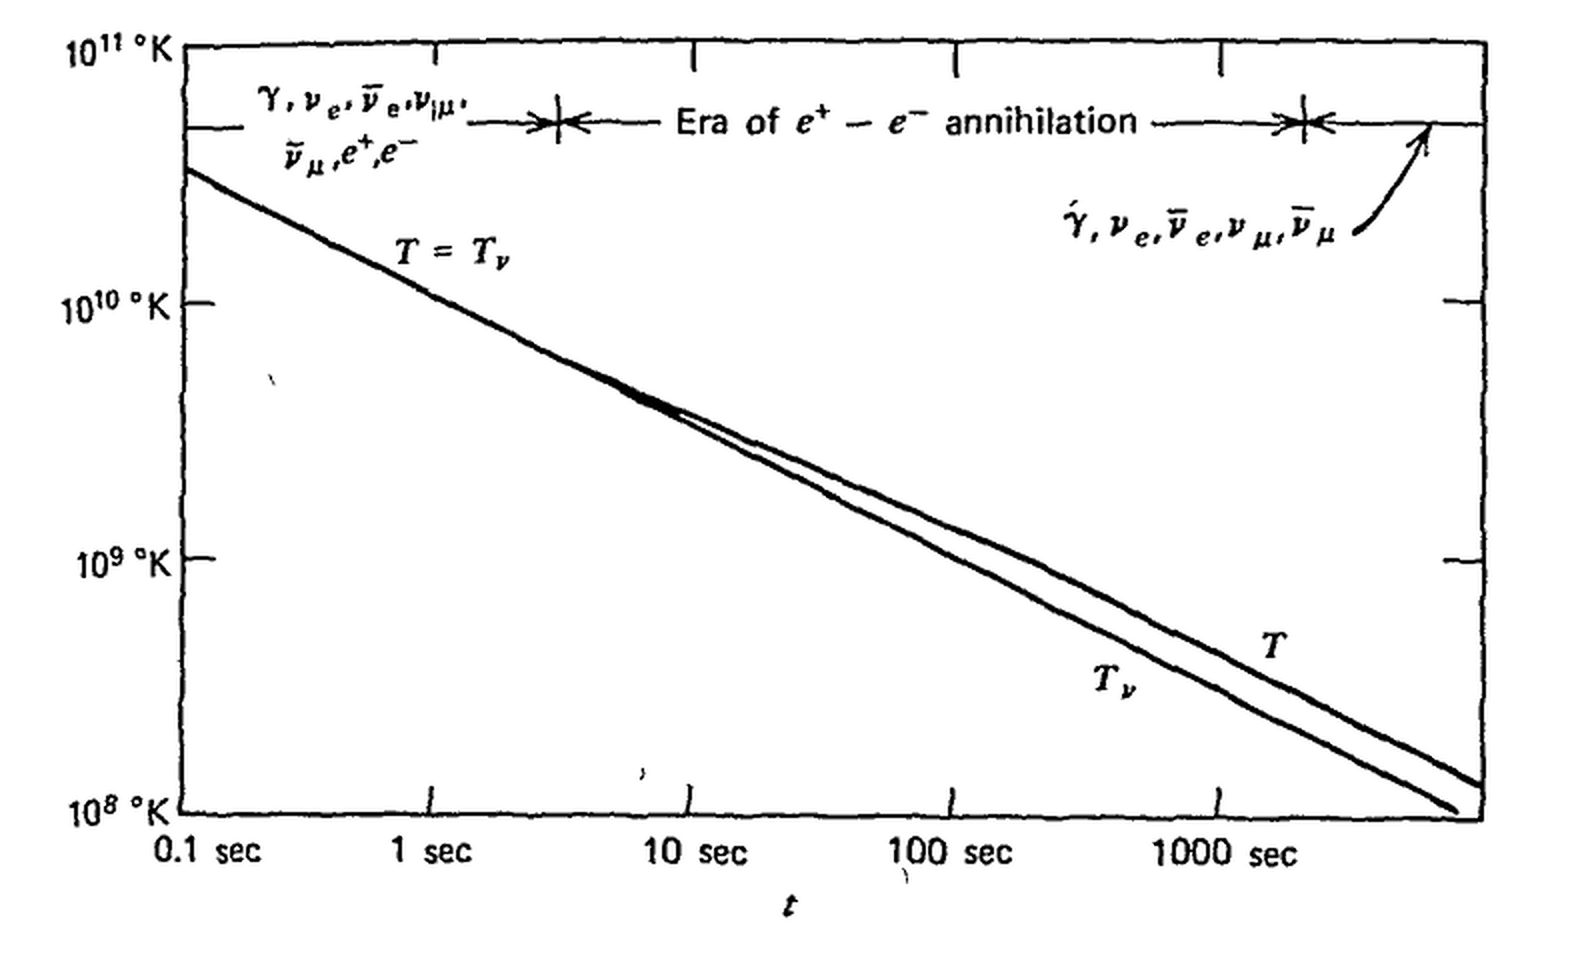
\includegraphics[width=0.92\linewidth]{figures/chapter15/fig15-05.png}
  \caption{Thermal history of the early universe. Here \(T\) is the
  temperature of the \(\gamma\)--\(e^+\)--\(e^-\) plasma, and \(T_\nu\) is
  the temperature of the decoupled
  \(\nu_e,\bar\nu_e,\nu_\mu,\bar\nu_\mu\).}
  \label{fig:15.5}
\end{figure}
\endgroup


\emph{(D)} As the temperature dropped below \(10^{11\,\circ}\mathrm K\)
(\(t\simeq0.01\,\mathrm{sec}\)), the neutron--proton mass difference began to
shift the small nucleonic contamination toward more protons and fewer neutrons.

\emph{(E)} As the temperature dropped below
\(5\times10^{9\,\circ}\mathrm K\) (\(t\simeq4\,\mathrm{sec}\)), the
electron--positron pairs began to annihilate, leaving as the dominant
constituents of the universe only photons, neutrinos, and antineutrinos in
essentially free expansion, with the photon temperature 40.1\% higher than the
neutrino temperature. At the same time, the cooling of the neutrinos and
antineutrinos, and the disappearance of the electrons and positrons, froze the
neutron--proton ratio at about \(1:5\).

\emph{(F)} At a temperature of about \(10^{9\,\circ}\mathrm K\)
(\(t\simeq180\,\mathrm{sec}\)), the neutrons rapidly began to fuse with protons
into heavier nuclei, leaving an ionized gas of hydrogen and
\(\mathrm{He}^4\), with about 27\% helium by weight, and a trace of
\(d\), \(\mathrm{He}^3\), and other elements.

\emph{(G)} The free expansion of the photons, neutrinos, and antineutrinos
continued, with \(T_\gamma=1.401T_\nu\propto a^{-1}\). The ionized gas
temperature remained locked to the photon temperature until the hydrogen
recombined at \(T\simeq4000^\circ\mathrm K\).

\emph{(H)} At some temperature between \(10^{5\,\circ}\mathrm K\) and
\(10^{8\,\circ}\mathrm K\), the energy density of the photons, neutrinos, and
antineutrinos dropped below the rest-mass density of hydrogen and helium, and
we entered upon the matter-dominated era.

In filling in the details of this history, it will prove very convenient to
concentrate in this section on the thermal evolution of the leading
constituents of the early universe, the photons and leptons, and postpone our
discussion of nucleosynthesis to the next section.

First, let us consider the equation governing the time scale for expansion of
the early universe. This is somewhat simpler than in the matter-dominated era,
because the curvature of space may be neglected. For \(k=\pm1\), the
right-hand side of the Einstein equation \eqref{eq:15.1.20} has a present value
given by Eqs.~\eqref{eq:15.2.5} and \eqref{eq:15.2.6},
\[
  \frac{8\pi G\rho_0a_0^2}{3}
  =
  \frac{2q_0}{\lvert 2q_0-1\rvert}.
\]
We saw in Section~\ref{sec:15.2} that \(q_0\) is probably greater than
0.014, so at present \(8\pi G\rho a^2/3\) is greater than 0.03. During the
matter-dominated era, this quantity varies as \(1/a\propto T_\gamma\), so it
was greater than 10 when \(T_\gamma\) was \(1000^\circ\mathrm K\), and was
even larger at earlier times. Hence, during the whole early history of the
universe, \(k\) was much less than the right-hand side of
Eq.~\eqref{eq:15.1.20}, and this equation therefore simplifies to
\begin{equation}
  \dot a^2=\frac{8\pi G\rho a^2}{3}.
  \tag{15.6.2}\label{eq:15.6.2}
\end{equation}
It will make no difference in our discussion of the early universe whether
space is open or closed.

Now we must consider what were the contents of the early universe. At any
given time, we can expect to find some particles in thermal equilibrium with
each other, other particles in free expansion, and perhaps some particles that
are just passing from one condition to the other. In the ideal-gas
approximation, the number density \(n_i(q)\dd q\) of particles of type \(i\)
with momentum between \(q\) and \(q+\dd q\) is given in thermal equilibrium by
a Fermi or a Bose distribution:\hyperref[ch15-ref-87]{\textsuperscript{87}}
\begin{equation}
  n_i(q)\dd q
  =
  4\pi h^{-3}g_iq^2\dd q
  \left[
    \exp\left(\frac{E_i(q)-\mu_i}{kT}\right)\pm1
  \right]^{-1},
  \tag{15.6.3}\label{eq:15.6.3}
\end{equation}
where \(E_i(q)=(m_i^2+q^2)^{1/2}\) is the particle energy, \(\mu_i\) is the
chemical potential, the sign \(\pm\) is \(+1\) for fermions and \(-1\) for
bosons, and \(g_i\) is the number of spin states, with \(g_i=1\) for neutrinos
and antineutrinos and \(g_i=2\) for photons, electrons, muons, nucleons, and
their antiparticles.

The chemical potentials must be determined from a consideration of the
conservation laws obeyed by the various possible
reactions.\hyperref[ch15-ref-88]{\textsuperscript{88}} The basic rule is that
\(\mu_i\) is additively conserved in all reactions. In particular:

\emph{(A)} Photons can be emitted or absorbed in an arbitrary reaction in any
number, so \(\mu_\gamma=0\). (Equation~\eqref{eq:15.6.3} then reduces to the
Planck distribution \eqref{eq:15.5.9}, with
\(n_\gamma=\rho_\gamma/h\nu\), \(g_\gamma=2\), and \(E_\gamma=h\nu\).)

\emph{(B)} Particle--antiparticle pairs can annihilate into photons, so the
chemical potentials of a particle and its antiparticle are equal and opposite.

\emph{(C)} Electrons and muons can be converted into their associated
neutrinos \(\nu_e\) and \(\nu_\mu\) by collisions with each other or with
nucleons, in such reactions as
\[
  e^-+p\rightleftarrows\nu_e+n,
  \qquad
  e^-+p\rightleftarrows\nu_\mu+n+\mu^-,
  \qquad
  \mu^-+p\rightleftarrows\nu_\mu+n,
  \quad\text{etc.}
\]
The chemical potentials are therefore related by
\begin{equation}
  \mu_{e^-}-\mu_{\nu_e}
  =
  \mu_{\mu^-}-\mu_{\nu_\mu}
  =
  \mu_n-\mu_p.
  \tag{15.6.4}\label{eq:15.6.4}
\end{equation}
Altogether there are just four independent conserved intrinsic quantum
numbers: charge, baryon number (nucleons and hyperons minus antinucleons and
antihyperons), electron-lepton number (\(e^-\) and \(\nu_e\) minus \(e^+\)
and \(\bar\nu_e\)), and muon-lepton
number\hyperref[ch15-ref-89]{\textsuperscript{89}} (\(\mu^-\) and \(\nu_\mu\)
minus \(\mu^+\) and \(\bar\nu_\mu\)). Hence there are just four independent
chemical potentials, which can be taken as
\(\mu_p,\mu_{e^-},\mu_{\nu_e},\mu_{\nu_\mu}\). These four independent chemical
potentials are to be determined by the values for the charge density \(N_Q\),
the baryon-number density \(N_B\), the electron-lepton-number density \(N_E\),
and the muon-lepton-number density \(N_M\), all of which simply vary as
\(a^{-3}\). The problem of determining the chemical potentials thus leads us
to the question: What are the values of the four densities
\(N_Q,N_B,N_E,N_M\)?

We know that the average charge density \(N_Q\) is zero, or at least very
small.\hyperref[ch15-ref-90]{\textsuperscript{90}} We also know that the baryon
number density \(N_B\) is much less than the number density \(n_\gamma\) of
photons, because at present
\(N_B\simeq n_p+n_n-n_{\bar p}-n_{\bar n}\) is 8 to 10 orders of magnitude
less than \(n_\gamma\), whereas at earlier times \(N_Ba^3\) was strictly
constant and \(n_\gamma a^3\propto(T_\gamma a)^3\) was roughly constant.
Unfortunately we know very little about the present number density of
neutrinos, so we cannot estimate the value of
\(N_E=n_{e^-}+n_{\nu_e}-n_{e^+}-n_{\bar\nu_e}\), or
\(N_M=n_{\mu^-}+n_{\nu_\mu}-n_{\mu^+}-n_{\bar\nu_\mu}\). However, since
\(N_B\) is 8 to 10 orders of magnitude less than \(n_\gamma\), it is at least
a reasonable guess that \(N_E\) and \(N_M\) are also much less than
\(n_\gamma\). If so, then it is a good approximation to set all the conserved
quantum numbers equal to zero:
\begin{equation}
  N_Q=N_B=N_E=N_M=0.
  \tag{15.6.5}\label{eq:15.6.5}
\end{equation}
Of course \(N_B\) is not really zero, and we shall have to put the baryons back
into the calculation in the next section when we consider the synthesis of the
elements, but they can be ignored in calculating the gross thermal history of
the early universe. The question of whether \(N_E\) and \(N_M\) can also be
ignored will be taken up at the end of this section.

The problem of determining the chemical potentials is now very easy. The
contributions of particles and antiparticles to the four densities
\(N_Q,N_B,N_E,N_M\) are equal and opposite, so the four densities are odd
functions of the four independent chemical potentials
\(\mu_p,\mu_{e^-},\mu_{\nu_e},\mu_{\nu_\mu}\). Hence the values of the
\(\mu_i\) determined by \eqref{eq:15.6.5} are simply
\begin{equation}
  \mu_i=0.
  \tag{15.6.6}\label{eq:15.6.6}
\end{equation}

This approximation allows us to deal with energy conservation in a very
convenient manner. The total energy density and pressure of all the particles
in thermal equilibrium are now evidently just functions of the temperature
alone:
\begin{align}
  \rho_{\mathrm{eq}}(T)
  &=
  \sum_i\int_0^\infty E_i(q)n_i(q;T)\dd q,
  \tag{15.6.7}\label{eq:15.6.7}\\
  p_{\mathrm{eq}}(T)
  &=
  \sum_i\int_0^\infty
  \frac{q^2}{3E_i(q)}n_i(q;T)\dd q.
  \tag{15.6.8}\label{eq:15.6.8}
\end{align}
[See Eqs.~\eqref{eq:2.10.21} and \eqref{eq:2.10.22}.] According to the second
law of thermodynamics, the entropy \(S\) of the particles in equilibrium at
temperature \(T\) within a volume \(V\) is a function \(S(V,T)\), with
\begin{equation}
  \dd S(V,T)
  =
  \frac1T\left\{
    \dd[\rho_{\mathrm{eq}}(T)V]+p_{\mathrm{eq}}(T)\dd V
  \right\},
  \tag{15.6.9}\label{eq:15.6.9}
\end{equation}
so that
\[
  \pd{S(V,T)}{V}
  =
  \frac1T[\rho_{\mathrm{eq}}(T)+p_{\mathrm{eq}}(T)],
  \qquad
  \pd{S(V,T)}{T}
  =
  \frac VT\od{\rho_{\mathrm{eq}}(T)}{T}.
\]
The energy density and pressure must then satisfy the integrability condition
\[
  \pd{}{T}\left\{
    \frac1T[\rho_{\mathrm{eq}}(T)+p_{\mathrm{eq}}(T)]
  \right\}
  =
  \pd{}{V}\left\{
    \frac VT\od{\rho_{\mathrm{eq}}(T)}{T}
  \right\},
\]
or, after a little rearrangement,
\begin{equation}
  \od{p_{\mathrm{eq}}(T)}{T}
  =
  \frac1T[\rho_{\mathrm{eq}}(T)+p_{\mathrm{eq}}(T)].
  \tag{15.6.10}\label{eq:15.6.10}
\end{equation}
[This may also be derived directly from Eqs.~\eqref{eq:15.6.7} and
\eqref{eq:15.6.8}.] As long as the particles in thermal equilibrium interact
only with each other, their total energy and pressure must separately satisfy
the energy-conservation equation \eqref{eq:14.2.19},
\begin{equation}
  \dot\rho_{\mathrm{eq}}
  =
  -3\frac{\dot a}{a}
  [\rho_{\mathrm{eq}}+p_{\mathrm{eq}}].
  \tag{15.6.11}\label{eq:15.6.11}
\end{equation}
Using \eqref{eq:15.6.10}, this may now be written
\begin{equation}
  \frac{\dd}{\dd t}
  \left\{
    \frac{a^3}{T}[\rho_{\mathrm{eq}}(T)+p_{\mathrm{eq}}(T)]
  \right\}
  =
  0.
  \tag{15.6.12}\label{eq:15.6.12}
\end{equation}
Thus conservation of energy has a simple interpretation in terms of the
entropy. Using \eqref{eq:15.6.10} in \eqref{eq:15.6.9} gives
\[
  \dd S(V,T)
  =
  \frac1T
  \dd\!\left\{
    [\rho_{\mathrm{eq}}(T)+p_{\mathrm{eq}}(T)]V
  \right\}
  -
  \frac{V}{T^2}
  [\rho_{\mathrm{eq}}(T)+p_{\mathrm{eq}}(T)]\dd T,
\]
so, except for a possible additive constant,
\begin{equation}
  S(V,T)
  =
  \frac VT[\rho_{\mathrm{eq}}(T)+p_{\mathrm{eq}}(T)].
  \tag{15.6.13}\label{eq:15.6.13}
\end{equation}
The result \eqref{eq:15.6.12} thus simply states the constancy of the entropy
in a volume \(a^3(t)\):
\begin{equation}
  s
  \equiv
  S(a^3,T)
  =
  \frac{a^3}{T}[\rho_{\mathrm{eq}}(T)+p_{\mathrm{eq}}(T)].
  \tag{15.6.14}\label{eq:15.6.14}
\end{equation}
In particular, when all the particles in equilibrium are highly relativistic,
we can set \(E_i=q\) in \eqref{eq:15.6.7} and \eqref{eq:15.6.8}, so that
\begin{equation}
  p_{\mathrm{eq}}(T)=\frac13\rho_{\mathrm{eq}}(T).
  \tag{15.6.15}\label{eq:15.6.15}
\end{equation}
Then Eq.~\eqref{eq:15.6.10} gives
\begin{equation}
  \rho_{\mathrm{eq}}(T)\propto T^4,
  \tag{15.6.16}\label{eq:15.6.16}
\end{equation}
with a ``constant'' of proportionality that depends on just which particle
types are abundant in equilibrium at these temperatures. [This result can
also be obtained directly from Eqs.~\eqref{eq:15.6.7} and
\eqref{eq:15.6.8}.] Using Eqs.~\eqref{eq:15.6.15} and
\eqref{eq:15.6.16} in \eqref{eq:15.6.12} then gives a temperature decrease
\begin{equation}
  T\propto\frac1a.
  \tag{15.6.17}\label{eq:15.6.17}
\end{equation}
We shall see that this holds through most, but not all, of the early history
of the universe.

Our next task is to decide which particles were in thermal equilibrium at
various times. One of the simplifications brought about by our neglect of the
chemical potentials is that the only particles that can be present in thermal
equilibrium with appreciable number densities \eqref{eq:15.6.3} are those with
mass \(m<kT\). For \(kT<m_\pi\), or
\(T<1.5\times10^{12\,\circ}\mathrm K\), these are the
\(\mu^\pm,e^\pm,\nu_e,\bar\nu_e,\nu_\mu,\bar\nu_\mu\), and \(\gamma\).
(Gravitons are ignored here, for reasons discussed in
Section~\ref{sec:15.11}.) Throughout the early history of the universe, the
processes of pair production and annihilation and Compton scattering kept any
extant charged particles in thermal equilibrium with the photons. Hence the
photons were described by the Planck law \eqref{eq:15.5.9}, and the \(e^\pm\)
and \(\mu^\pm\) were described by Fermi distributions with zero chemical
potential:
\begin{align}
  n_{e^-}(q)\dd q
  =
  n_{e^+}(q)\dd q
  &=
  8\pi h^{-3}q^2\dd q
  \left[
    \exp\left(\frac{\sqrt{q^2+m_e^2}}{kT}\right)+1
  \right]^{-1},
  \tag{15.6.18}\label{eq:15.6.18}\\
  n_{\mu^-}(q)\dd q
  =
  n_{\mu^+}(q)\dd q
  &=
  8\pi h^{-3}q^2\dd q
  \left[
    \exp\left(\frac{\sqrt{q^2+m_\mu^2}}{kT}\right)+1
  \right]^{-1}.
  \tag{15.6.19}\label{eq:15.6.19}
\end{align}

What about the neutrinos and antineutrinos? We know that they can be produced,
destroyed, and scattered in reactions such as
\begin{equation}
  \begin{gathered}
    e^-+\mu^+\rightleftarrows\nu_e+\bar\nu_\mu,
    \qquad
    e^++\mu^-\rightleftarrows\bar\nu_e+\nu_\mu,
    \\
    \nu_e+\mu^-\rightleftarrows\nu_\mu+e^-,
    \qquad
    \bar\nu_e+\mu^+\rightleftarrows\bar\nu_\mu+e^+,
    \\
    \nu_\mu+\mu^+\rightleftarrows\nu_e+e^+,
    \qquad
    \bar\nu_\mu+\mu^-\rightleftarrows\bar\nu_e+e^-.
  \end{gathered}
  \tag{15.6.20}\label{eq:15.6.20}
\end{equation}
As long as \(kT<m_\mu\), the cross sections for all of these reactions will be
roughly of order
\begin{equation}
  \sigma_{\mathrm{wk}}
  \simeq
  g_{\mathrm{wk}}^2\hbar^{-4}(kT)^2,
  \tag{15.6.21}\label{eq:15.6.21}
\end{equation}
where \(g_{\mathrm{wk}}=1.4\times10^{-49}\,\mathrm{erg\,cm^3}\) is the weak
coupling constant, known from the observed rate for the muon decay process
\(\mu^-\to e^-+\nu_\mu+\bar\nu_e\). At these temperatures all particle
velocities are of order unity, and Eqs.~\eqref{eq:15.6.18} and
\eqref{eq:15.6.19} give the densities of the charged leptons \(e^\pm\) and
\(\mu^\pm\) as
\begin{equation}
  n_\ell\simeq\left(\frac{kT}{\hbar}\right)^3.
  \tag{15.6.22}\label{eq:15.6.22}
\end{equation}
Hence the rate at which a single neutrino is scattered, and the rate of
neutrino production per charged lepton, are both of order
\begin{equation}
  \sigma_{\mathrm{wk}}n_\ell
  \simeq
  g_{\mathrm{wk}}^2\hbar^{-7}(kT)^5.
  \tag{15.6.23}\label{eq:15.6.23}
\end{equation}
The total energy density is roughly of order
\begin{equation}
  \rho\simeq kT\left(\frac{kT}{\hbar}\right)^3,
  \tag{15.6.24}\label{eq:15.6.24}
\end{equation}
so according to Eq.~\eqref{eq:15.6.2}, the expansion rate is of order
\begin{equation}
  H\equiv\frac{\dot a}{a}
  \simeq
  (G\rho)^{1/2}
  \simeq
  G^{1/2}\hbar^{-3/2}(kT)^2.
  \tag{15.6.25}\label{eq:15.6.25}
\end{equation}
Hence, as long as \(kT>m_\mu\), or \(T>10^{12\,\circ}\mathrm K\), the ratio
of the reaction rate \(\sigma n_\ell\) to the expansion rate \(H\) is (now
using c.g.s.\ units)
\begin{equation}
  \frac{\sigma n_\ell}{H}
  \simeq
  G^{-1/2}\hbar^{-11/2}g_{\mathrm{wk}}^2(kT)^3
  \simeq
  \left(\frac{T}{10^{10\,\circ}\mathrm K}\right)^3.
  \tag{15.6.26}\label{eq:15.6.26}
\end{equation}
However, all of the reactions \eqref{eq:15.6.20} require either the presence
of a \(\mu^-\) or \(\mu^+\), or enough energy to make a \(\mu^-\) or
\(\mu^+\). When \(kT<m_\mu\), the number density of muons, and the number
densities of other particles with energy \(E>m_\mu\), are reduced by factors
of order \(\exp(-m_\mu/kT)\), and in consequence the ratio of the reaction
rate to the expansion rate is of order
\begin{equation}
  \frac{\sigma n_\ell}{H}
  \simeq
  \left(\frac{T}{10^{10\,\circ}\mathrm K}\right)^3
  \exp\left(-\frac{10^{12\,\circ}\mathrm K}{T}\right).
  \tag{15.6.27}\label{eq:15.6.27}
\end{equation}
The neutrinos and antineutrinos drop out of thermal equilibrium with the other
particles when this ratio falls below unity, that is, at about
\(T\simeq1.3\times10^{11\,\circ}\mathrm K\).

Actually, it may be that the \(\nu_e\) and \(\bar\nu_e\) remain in thermal
equilibrium a little longer than the \(\nu_\mu\) and \(\bar\nu_\mu\).
According to present theories,\hyperref[ch15-ref-91]{\textsuperscript{91}} the
weak interactions arise from the coupling of a ``weak current'' to itself,
either directly, or through the agency of a charged spin-1 particle, the
``intermediate vector meson.'' If this is so, then there are additional
reactions involving \(\nu_e\) and \(\bar\nu_e\),
\begin{equation}
  e^-+e^+\rightleftarrows\nu_e+\bar\nu_e,
  \qquad
  e^\pm+\nu_e\to e^\pm+\nu_e,
  \qquad
  e^\pm+\bar\nu_e\to e^\pm+\bar\nu_e,
  \tag{15.6.28}\label{eq:15.6.28}
\end{equation}
whose cross sections are of order \eqref{eq:15.6.21} for \(kT>m_e\). These
reactions do not involve \(\mu^\pm\), so the ratio of the \(\nu_e\) and
\(\bar\nu_e\) reaction rates to the expansion rate \(H\) would be given by
Eq.~\eqref{eq:15.6.26} for \(kT>m_e\), that is, down to a temperature
\(T\simeq5\times10^{9\,\circ}\mathrm K\). The reactions \eqref{eq:15.6.28}
could then keep \(\nu_e\) and \(\bar\nu_e\) in thermal equilibrium with
\(\gamma\) and \(e^\pm\) down to a temperature
\(T\simeq10^{10\,\circ}\mathrm K\), where the ratio \eqref{eq:15.6.26} drops
to unity. The same may even be
true\hyperref[ch15-ref-173]{\textsuperscript{173}} for \(\nu_\mu\) and
\(\bar\nu_\mu\).

We are now in a position to work out the thermal history of the early
universe. Let us start at a temperature between \(10^{12\,\circ}\mathrm K\)
and \(1.3\times10^{11\,\circ}\mathrm K\), when the \(\mu^+\) and \(\mu^-\)
were rare enough so that their contribution to \(\rho_{\mathrm{eq}}\) and
\(p_{\mathrm{eq}}\) could be neglected, and yet abundant enough to keep the
neutrinos and antineutrinos in thermal equilibrium with the other particles.
The important constituents of the universe then were
\(e^\pm,\gamma,\nu_e,\bar\nu_e,\nu_\mu,\bar\nu_\mu\), all in thermal
equilibrium. The photons had a Planck distribution, the \(e^\pm\) had the
Fermi distribution \eqref{eq:15.6.18}, and the neutrinos and antineutrinos had
the Fermi distribution
\begin{align}
  n_{\nu_e}(q)\dd q
  =
  n_{\bar\nu_e}(q)\dd q
  &=
  n_{\nu_\mu}(q)\dd q
  =
  n_{\bar\nu_\mu}(q)\dd q
  \notag\\
  &=
  4\pi h^{-3}q^2\dd q
  \left[\exp\left(\frac q{kT}\right)+1\right]^{-1}.
  \tag{15.6.29}\label{eq:15.6.29}
\end{align}
Since all these particles were highly relativistic, the temperature was
falling in obedience to Eq.~\eqref{eq:15.6.17}, that is,
\(T\propto a^{-1}\). When \(T\) dropped to about
\(1.3\times10^{11\,\circ}\mathrm K\), the \(\nu_\mu\) and \(\bar\nu_\mu\),
and possibly also the \(\nu_e\) and \(\bar\nu_e\), decoupled from the particles
in equilibrium and began a free expansion. \emph{However, this decoupling had
no effect on any of the distribution functions.} The particles remaining in
equilibrium still constituted a highly relativistic gas, so their temperature
continued to drop like \(1/a\). In addition, the number density of the free
neutrinos and antineutrinos fell like \(1/a^3\) and their momenta were
red-shifted by a factor \(1/a\) (just as for photons), so that the form of the
distribution \eqref{eq:15.6.29} was preserved, with a neutrino temperature
\(T_\nu\) proportional to \(1/a\). Since \(T_\nu\) equaled \(T\) before
decoupling, and \(T_\nu\) and \(T\) both decreased like \(1/a\) thereafter,
the neutrinos and antineutrinos continued to be described by the Fermi
distribution \eqref{eq:15.6.29} with \(T_\nu=T\), just as if they had remained
in thermal equilibrium with the other particles. There may have been a second
decoupling, of \(\nu_e\) and \(\bar\nu_e\) at
\(T\simeq10^{10\,\circ}\mathrm K\), but again this made no difference to the
neutrino and antineutrino distribution function provided that they, and
\(\nu_\mu,\bar\nu_\mu\), mostly decoupled while the \(e^\pm\) were still
relativistic. Thus, during the whole of the era
\(10^{11\,\circ}\mathrm K>T>5\times10^{9\,\circ}\mathrm K\), the neutrinos
and antineutrinos behaved as if they were in thermal equilibrium, and all
particles, \(\gamma,e^\pm,\nu_e,\bar\nu_e,\nu_\mu,\bar\nu_\mu\), were
described by Planck or Fermi distributions with the same temperature \(T\),
falling like \(1/a\). The energy densities of the neutrinos and antineutrinos
were thus
\begin{equation}
  \rho_{\nu_e}
  =
  \rho_{\bar\nu_e}
  =
  \rho_{\nu_\mu}
  =
  \rho_{\bar\nu_\mu}
  \equiv
  \rho_\nu,
  \tag{15.6.30}\label{eq:15.6.30}
\end{equation}
where
\begin{align}
  \rho_\nu
  &=
  4\pi h^{-3}\int_0^\infty
  q^3\left[\exp\left(\frac q{kT}\right)+1\right]^{-1}\dd q
  \notag\\
  &=
  \frac{7\pi^5}{30h^3}(kT)^4
  =
  \frac7{16}a_{\mathrm{rad}}T^4.
  \tag{15.6.31}\label{eq:15.6.31}
\end{align}
Also, for \(kT>m_e\), the \(e^\pm\) were relativistic, so
\begin{equation}
  \rho_{e^-}
  =
  \rho_{e^+}
  =
  2\rho_\nu
  =
  \frac78a_{\mathrm{rad}}T^4.
  \tag{15.6.32}\label{eq:15.6.32}
\end{equation}
(The densities \(\rho_{e^\pm}\) are twice \(\rho_\nu\) because the \(e^-\)
and \(e^+\) each have two spin states.) The total energy density of the
universe during the era from \(T<10^{12\,\circ}\mathrm K\) to
\(T\simeq10^{10\,\circ}\mathrm K\) was thus
\begin{align}
  \rho
  &=
  \rho_{\nu_e}+\rho_{\bar\nu_e}
  +\rho_{\nu_\mu}+\rho_{\bar\nu_\mu}
  +\rho_{e^-}+\rho_{e^+}+\rho_\gamma
  \notag\\
  &=
  \frac92a_{\mathrm{rad}}T^4.
  \tag{15.6.33}\label{eq:15.6.33}
\end{align}

The story now becomes a little more complicated. Below \(10^{10\,\circ}\mathrm
K\), the only important particles left in thermal equilibrium were the
\(e^\pm\) and \(\gamma\). Their entropy per volume \(a^3\) is given by
Eqs.~\eqref{eq:15.6.14}, \eqref{eq:15.6.7}, \eqref{eq:15.6.8}, and
\eqref{eq:15.6.18}:
\begin{equation}
  s
  =
  \frac{a^3}{T}
  [\rho_{e^-}+\rho_{e^+}+\rho_\gamma
  +p_{e^-}+p_{e^+}+p_\gamma].
  \tag{15.6.34}\label{eq:15.6.34}
\end{equation}
For \(T>5\times10^{9\,\circ}\mathrm K\), the electrons and positrons were
relativistic, so Eqs.~\eqref{eq:15.6.15} and \eqref{eq:15.6.32} apply, and
Eq.~\eqref{eq:15.6.34} gives
\begin{equation}
  s
  =
  \frac{4a^3}{3T}
  [\rho_{e^-}+\rho_{e^+}+\rho_\gamma]
  =
  \frac{11}{3}a_{\mathrm{rad}}(aT)^3.
  \tag{15.6.35}\label{eq:15.6.35}
\end{equation}
As \(T\) dropped below \(5\times10^{9\,\circ}\mathrm K\), the \(e^+\) and
\(e^-\) annihilated, eventually leaving just photons, with
\begin{equation}
  s
  =
  \frac{4a^3}{3T}\rho_\gamma
  =
  \frac43a_{\mathrm{rad}}(aT)^3.
  \tag{15.6.36}\label{eq:15.6.36}
\end{equation}
But \(s\) is constant, so the effect of the disappearance of \(e^-\) and
\(e^+\) was to increase \(aT\) by a factor
\begin{equation}
  \frac{(aT)_{T<10^{9\,\circ}\mathrm K}}
       {(aT)_{T>5\times10^{9\,\circ}\mathrm K}}
  =
  \left(\frac{11}{4}\right)^{1/3}.
  \tag{15.6.37}\label{eq:15.6.37}
\end{equation}

The neutrinos and antineutrinos did not get heated by the electron--positron
annihilation, so their temperature just continued to fall like \(a^{-1}\).
Hence, for \(T<5\times10^{9\,\circ}\mathrm K\), we have to distinguish
between the temperature \(T_\nu\) of the neutrinos and antineutrinos, and the
temperature \(T\) of the photons plus any remaining charged particles. Since
\(aT_\nu\) is constant and \(aT\) jumped by the factor
\((11/4)^{1/3}\), the photon temperature was eventually greater than the
neutrino temperature by just this factor:
\begin{equation}
  \left(\frac{T}{T_\nu}\right)_{T<10^{9\,\circ}\mathrm K}
  =
  \left(\frac{11}{4}\right)^{1/3}
  =
  1.401.
  \tag{15.6.38}\label{eq:15.6.38}
\end{equation}
In order to determine the behavior of \(aT\) or \(T/T_\nu\) between
\(5\times10^{9\,\circ}\mathrm K\) and \(10^{9\,\circ}\mathrm K\), we have to
use the expression \eqref{eq:15.6.34}, or
\begin{equation}
  s
  =
  \frac43a_{\mathrm{rad}}(aT)^3
  \mathscr S\left(\frac{m_e}{kT}\right),
  \tag{15.6.39}\label{eq:15.6.39}
\end{equation}
where
\begin{align}
  \mathscr S(x)
  &=
  1+\frac{45}{2\pi^4}
  \int_0^\infty y^2\dd y
  \left[
    \sqrt{x^2+y^2}
    +
    \frac{y^2}{3\sqrt{x^2+y^2}}
  \right]
  \notag\\
  &\qquad\times
  \left[\exp\left(\sqrt{x^2+y^2}\right)+1\right]^{-1}.
  \tag{15.6.40}\label{eq:15.6.40}
\end{align}
The constant \(s\) can be expressed in terms of the constant \(aT_\nu\) by
replacing \(T\) with \(T_\nu\) in \eqref{eq:15.6.35}, so that
\begin{equation}
  T_\nu
  =
  \left(\frac4{11}\right)^{1/3}
  T
  \left[
    \mathscr S\left(\frac{m_e}{kT}\right)
  \right]^{1/3}.
  \tag{15.6.41}\label{eq:15.6.41}
\end{equation}
A numerical calculation\hyperref[ch15-ref-93]{\textsuperscript{93}} of the
function \(\mathscr S\) shows that \(T/T_\nu\) had risen only to 1.001 by the
time the temperature dropped to \(3\times10^{9\,\circ}\mathrm K\), and
\(T/T_\nu\) did not reach 1.4 until \(T\) fell below
\(10^{9\,\circ}\mathrm K\). (See Table~\ref{tab:15.4}.)

For \(T<10^{9\,\circ}\mathrm K\), the only particles in thermal equilibrium
with the photons were the small number of nucleons and electrons left over
after all the \(e^-e^+\) pairs annihilated. Both \(T_\nu\) and \(T\)
continued to fall like \(1/a\), with a ratio fixed at the value
\eqref{eq:15.6.37}. We saw in the last section that the photon temperature
\(T_\gamma\) began to differ from the matter temperature \(T\) after \(T\)
dropped below \(4000^\circ\mathrm K\), but the photon temperature continued
thereafter to drop like \(1/a\). Thus there should now be a cosmic
``black-body'' neutrino and antineutrino background described by
Eq.~\eqref{eq:15.6.29}, with temperature
\[
  T_{\nu0}
  =
  \left(\frac4{11}\right)^{1/3}T_{\gamma0}
  =
  1.9^\circ\mathrm K.
\]
From the time when \(T\simeq10^{9\,\circ}\mathrm K\) until the present, the
energy density of the photons, neutrinos, and antineutrinos has been
\begin{align}
  \rho_R
  &\equiv
  \rho_\gamma+\rho_{\nu_e}+\rho_{\bar\nu_e}
  +\rho_{\nu_\mu}+\rho_{\bar\nu_\mu}
  \notag\\
  &=
  a_{\mathrm{rad}}T_\gamma^4
  +
  \frac74a_{\mathrm{rad}}T_\nu^4
  \notag\\
  &=
  \left[
    1+\frac74\left(\frac4{11}\right)^{4/3}
  \right]a_{\mathrm{rad}}T_\gamma^4
  =
  1.45a_{\mathrm{rad}}T_\gamma^4.
  \tag{15.6.42}\label{eq:15.6.42}
\end{align}

This may be compared with the energy density \(m_Nn_N\) of nonrelativistic
matter, which scales as \(a^{-3}\), or \(T_\gamma^3\):
\[
  n_N
  =
  n_{N0}\left(\frac{T_\gamma}{T_{\gamma0}}\right)^3.
\]
Hence the critical temperature \(T_c\), at which \(m_Nn_N\) equaled
\(\rho_R\), is
\begin{equation}
  T_c
  =
  \frac{m_Nn_{N0}}{1.45a_{\mathrm{rad}}T_{\gamma0}^3}
  =
  4200^\circ\mathrm K
  \left[
    \frac{m_Nn_{N0}}{10^{-30}\,\mathrm{g/cm^3}}
  \right].
  \tag{15.6.43}\label{eq:15.6.43}
\end{equation}
For \(m_Nn_{N0}\) in the range \(2\times10^{-29}\,\mathrm{g/cm^3}\) to
\(3\times10^{-31}\,\mathrm{g/cm^3}\), this temperature lies in the range
\(84{,}000^\circ\mathrm K\) to \(1200^\circ\mathrm K\). It may be noted that
the temperature \(T_R\simeq4000^\circ\mathrm K\), at which ionized hydrogen
recombined, lies within this range, so we are not certain whether the energy
density of radiation was greater or less than that of matter at the time when
matter and radiation lost thermal contact. This uncertainty did not affect our
discussion of the microwave background in the last section; the important
point there was that the number density of photons is and was much greater
than that of baryons.

How long does all this take? During the era when the temperature was between
about \(10^{12\,\circ}\mathrm K\) and \(5\times10^{9\,\circ}\mathrm K\), and
also after it dropped below about \(10^{9\,\circ}\mathrm K\), the only
particles present in large numbers were all highly relativistic, so that
\(p=\rho/3\). According to Eq.~\eqref{eq:15.1.23}, the energy density
\(\rho\) varied as
\[
  \rho\propto a^{-4}.
\]
During these periods, the dynamical equation \eqref{eq:15.6.2} may be written
\[
  \frac{\dot\rho}{\rho}
  =
  -4\frac{\dot a}{a}
  =
  -4\left(\frac{8\pi G\rho}{3}\right)^{1/2}.
\]
The solution is
\begin{equation}
  t
  =
  \left(\frac{3}{32\pi G\rho}\right)^{1/2}
  +\text{constant}.
  \tag{15.6.44}\label{eq:15.6.44}
\end{equation}
During the period when
\(10^{12\,\circ}\mathrm K>T>5\times10^{9\,\circ}\mathrm K\), the energy
density was given by Eq.~\eqref{eq:15.6.33}, so that (using c.g.s.\ units)
\[
  \begin{split}
    t
    &=
    \left(
      \frac{c^2}{48\pi G a_{\mathrm{rad}}T^4}
    \right)^{1/2}
    +\text{constant}
    \\
    &=
    1.00\,\mathrm{sec}
    \left[
      \frac{T}{10^{10\,\circ}\mathrm K}
    \right]^{-2}
    +\text{constant}.
  \end{split}
\]
Starting at \(T=10^{12\,\circ}\mathrm K\), it took 0.0107 sec for the
temperature to relax to \(10^{11\,\circ}\mathrm K\), and another 1.07 sec for
the temperature to drop to \(10^{10\,\circ}\mathrm K\).

During the period when \(10^{9\,\circ}\mathrm K>T>T_c\), the energy density
was given by Eq.~\eqref{eq:15.6.42}, so that
\[
  \begin{split}
    t
    &=
    \left(
      \frac{c^2}{15.5\pi G a_{\mathrm{rad}}T_\gamma^4}
    \right)^{1/2}
    +\text{constant}
    \\
    &=
    1.92\,\mathrm{sec}
    \left[
      \frac{T_\gamma}{10^{10\,\circ}\mathrm K}
    \right]^{-2}
    +\text{constant}.
  \end{split}
\]
The time required for the temperature to drop from
\(10^{9\,\circ}\mathrm K\) to \(10^{8\,\circ}\mathrm K\) was thus about
5.3 hr. If radiation continued to dominate over matter until the hydrogen
recombined at \(T=4000^\circ\mathrm K\), then the age of the universe at the
time of recombination was \(4\times10^5\) years.

Unfortunately, if we want to describe the behavior of \(T(t)\) and \(a(t)\)
throughout the whole early history of the universe, we have to do a numerical
calculation to get through the era of electron--positron annihilation. In order
to express \(a\) in terms of \(T\), we use the fact that \eqref{eq:15.6.39}
was constant from \(T<10^{12\,\circ}\mathrm K\) until the present, provided
that after \(T\) dropped to \(4000^\circ\mathrm K\), we replace \(T\) with
\(T_\gamma\). Thus
\begin{equation}
  s
  =
  \frac43a_{\mathrm{rad}}(a_0T_{\gamma0})^3,
  \tag{15.6.45}\label{eq:15.6.45}
\end{equation}
and Eq.~\eqref{eq:15.6.39} can therefore be written
\begin{equation}
  \frac{a}{a_0}
  =
  \left(\frac{T}{T_{\gamma0}}\right)^{-1}
  \mathscr S^{-1/3}\left(\frac{m_e}{kT}\right).
  \tag{15.6.46}\label{eq:15.6.46}
\end{equation}
The energy density \(\rho\) is a function of \(T\), which, for \(T\) less
than \(10^{12\,\circ}\mathrm K\) and greater than both \(T_c\) and
\(4000^\circ\mathrm K\), may be written
\begin{align*}
  \rho
  &=
  \rho_\gamma+\rho_{\nu_e}+\rho_{\bar\nu_e}
  +\rho_{\nu_\mu}+\rho_{\bar\nu_\mu}
  +\rho_{e^+}+\rho_{e^-}
  \\
  &=
  a_{\mathrm{rad}}T^4
  +\frac74a_{\mathrm{rad}}T_\nu^4
  +16\pi h^{-3}\int_0^\infty
  E_e(q)q^2
  \left[
    \exp\left(\frac{E_e(q)}{kT}\right)+1
  \right]^{-1}\dd q.
\end{align*}
Using Eq.~\eqref{eq:15.6.41} for \(T_\nu\), this is
\begin{equation}
  \rho
  =
  a_{\mathrm{rad}}T^4
  \mathscr E\left(\frac{m_e}{kT}\right),
  \tag{15.6.47}\label{eq:15.6.47}
\end{equation}
where
\begin{align}
  \mathscr E(x)
  &=
  1
  \frac74\left(\frac4{11}\right)^{4/3}
  \mathscr S^{4/3}(x)
  \notag\\
  &\quad
  +
  \frac{30}{\pi^4}\int_0^\infty
  \sqrt{x^2+y^2}\,y^2\dd y
  \left[
    \exp\left(\sqrt{x^2+y^2}\right)+1
  \right]^{-1}.
  \tag{15.6.48}\label{eq:15.6.48}
\end{align}
Equations~\eqref{eq:15.6.46} and \eqref{eq:15.6.47} can be used in the
dynamical equation \eqref{eq:15.6.2},
\[
  \dd t
  =
  \left(\frac{8\pi G\rho}{3}\right)^{-1/2}
  \frac{\dd a}{a},
\]
and we find a formula for the time as a function of the temperature:
\begin{equation}
  t
  =
  -\int
  \left\{
    \frac{8\pi G a_{\mathrm{rad}}T^4
    \mathscr E(m_e/kT)}{3}
  \right\}^{-1/2}
  \left\{
    \frac{\dd T}{T}
    +
    \frac{\dd\mathscr S(m_e/kT)}
         {3\mathscr S(m_e/kT)}
  \right\}.
  \tag{15.6.49}\label{eq:15.6.49}
\end{equation}
Results\hyperref[ch15-ref-93]{\textsuperscript{93}} for \(t\), \(a/a_0\),
and \(T/T_\nu\), as functions of \(T\), are given in Table~\ref{tab:15.4}.

\begingroup
\renewcommand{\thetable}{15.4}
\begin{table}[htbp]
  \centering
  \caption{Thermal History of the Universe, from the Annihilation of
  \(\mu^+\mu^-\) Pairs Until the Decoupling of Matter and Radiation.}
  \label{tab:15.4}
  \small
  \begin{tabular}{@{}rrrr@{}}
    \toprule
    \(T\) (\(^{\circ}\mathrm K\)) &
    \(a/a_0\) &
    \(T/T_\nu\) &
    \(t\) (sec) \\
    \midrule
    \(10^{12}\)            & \(1.9\times10^{-12}\) & 1.000 & \(0\) \\
    \(6\times10^{11}\)     & \(3.2\times10^{-12}\) & 1.000 & \(1.94\times10^{-4}\) \\
    \(3\times10^{11}\)     & \(6.4\times10^{-12}\) & 1.000 & \(1.129\times10^{-3}\) \\
    \(2\times10^{11}\)     & \(9.6\times10^{-12}\) & 1.000 & \(2.61\times10^{-3}\) \\
    \(10^{11}\)            & \(1.9\times10^{-11}\) & 1.000 & \(1.078\times10^{-2}\) \\
    \(6\times10^{10}\)     & \(3.2\times10^{-11}\) & 1.000 & \(3.01\times10^{-2}\) \\
    \(3\times10^{10}\)     & \(6.4\times10^{-11}\) & 1.001 & \(0.1209\) \\
    \(2\times10^{10}\)     & \(9.6\times10^{-11}\) & 1.002 & \(0.273\) \\
    \(10^{10}\)            & \(1.9\times10^{-10}\) & 1.008 & \(1.103\) \\
    \(6\times10^9\)        & \(3.1\times10^{-10}\) & 1.022 & \(3.14\) \\
    \(3\times10^9\)        & \(5.9\times10^{-10}\) & 1.081 & \(13.83\) \\
    \(2\times10^9\)        & \(8.3\times10^{-10}\) & 1.159 & \(35.2\) \\
    \(10^9\)               & \(2.6\times10^{-9}\)  & 1.346 & \(1.82\times10^2\) \\
    \(3\times10^8\)        & \(9.0\times10^{-9}\)  & 1.401 & \(2.08\times10^3\) \\
    \(10^8\)               & \(2.7\times10^{-8}\)  & 1.401 & \(1.92\times10^4\) \\
    \(10^7\)               & \(2.7\times10^{-7}\)  & 1.401 & \(1.92\times10^6\) \\
    \(10^6\)               & \(2.7\times10^{-6}\)  & 1.401 & \(1.92\times10^8\) \\
    \(10^5\)               & \(2.7\times10^{-5}\)  & 1.401 & \(1.92\times10^{10}\) \\
    \(10^4\)               & \(2.7\times10^{-4}\)  & 1.401 & \(1.92\times10^{12}\) \\
    \(4\times10^3\)        & \(6.3\times10^{-4}\)  & 1.401 & \(1.20\times10^{13}\) \\
    \bottomrule
  \end{tabular}

  \vspace{0.5em}
  \begin{minipage}{0.94\linewidth}
    \footnotesize
    The values for \(a/a_0\) are derived assuming a present radiation
    temperature \(T_{\gamma0}=2.7^\circ\mathrm K\). The last two values for
    \(t\) are derived under the assumption that the energy density of matter
    was still negligible compared with that of photons and neutrinos. Values
    of \(T/T_\nu\), and \(t\) for \(T>10^{8\,\circ}\mathrm K\), are taken
    from F.~J.~E. Peebles, \emph{Ap.\ J.} \textbf{146}, 542 (1966).
  \end{minipage}
\end{table}
\endgroup

The only really arbitrary assumption so far has been the conjecture that the
lepton-number densities \(N_E\) and \(N_M\) are zero, or at least much less
than \(n_\gamma\). Let us now consider what would be the effect of giving up
this assumption. Once the temperature had dropped below
\(10^{12\,\circ}\mathrm K\), the only abundant charged particles were the
electrons and positrons, so charge neutrality required that
\(N_Q=n_{e^+}-n_{e^-}\) vanished. The chemical potential of the electron must
then have vanished, so the only particles that might then have had nonvanishing
chemical potentials were the neutrinos and antineutrinos. For
\(T>1.3\times10^{11\,\circ}\mathrm K\), these particles were in equilibrium
with \(\gamma,e^+\), and \(e^-\), so they were described by the Fermi
distributions
\begin{align}
  n_{\nu_e}(q)\dd q
  &=
  4\pi h^{-3}q^2\dd q
  \left[
    \exp\left(\frac{q-\mu_{\nu_e}}{kT}\right)+1
  \right]^{-1},
  \tag{15.6.50}\label{eq:15.6.50}\\
  n_{\bar\nu_e}(q)\dd q
  &=
  4\pi h^{-3}q^2\dd q
  \left[
    \exp\left(\frac{q+\mu_{\nu_e}}{kT}\right)+1
  \right]^{-1},
  \tag{15.6.51}\label{eq:15.6.51}
\end{align}
and likewise for \(\nu_\mu\) and \(\bar\nu_\mu\). The lepton-number densities
were then
\begin{align}
  N_E
  &=
  \int_0^\infty
  [n_{\nu_e}(q)-n_{\bar\nu_e}(q)]\dd q
  =
  4\pi\left(\frac{kT}{h}\right)^3
  \mathscr N\left(\frac{\mu_{\nu_e}}{kT}\right),
  \tag{15.6.52}\label{eq:15.6.52}\\
  N_M
  &=
  \int_0^\infty
  [n_{\nu_\mu}(q)-n_{\bar\nu_\mu}(q)]\dd q
  =
  4\pi\left(\frac{kT}{h}\right)^3
  \mathscr N\left(\frac{\mu_{\nu_\mu}}{kT}\right),
  \tag{15.6.53}\label{eq:15.6.53}
\end{align}
where
\begin{equation}
  \mathscr N(x)
  \equiv
  \int_0^\infty
  \left\{
    [e^{y-x}+1]^{-1}
    -
    [e^{y+x}+1]^{-1}
  \right\}y^2\dd y.
  \tag{15.6.54}\label{eq:15.6.54}
\end{equation}
Since electron-lepton number and muon-lepton number are believed to be
conserved,\hyperref[ch15-ref-89]{\textsuperscript{89}} the densities \(N_E\)
and \(N_M\) must always vary as \(a^{-3}\). However, we have seen that during
the era when
\(10^{12\,\circ}\mathrm K>T>5\times10^{9\,\circ}\mathrm K\), \(T\) varies
as \(1/a\). Hence \(\mu_{\nu_e}/kT\) and \(\mu_{\nu_\mu}/kT\) must have been
constant, from the annihilation of the \(\mu^+\) and \(\mu^-\) until the
decoupling of the neutrinos and antineutrinos.

After decoupling, the neutrinos and antineutrinos have expanded freely, with
number densities dropping as \(1/a^3\) and momenta red-shifted by a factor
\(1/a\). This free expansion preserved the form of the distributions
\eqref{eq:15.6.50} and \eqref{eq:15.6.51}, but red-shifted the temperature and
the chemical potentials by a factor \(1/a\). Hence the neutrino distributions,
during the whole period from \(T<10^{12\,\circ}\mathrm K\) until the present,
are given by
\begin{align}
  n_{\nu_e}(q)\dd q
  &=
  4\pi h^{-3}q^2\dd q
  \left[
    \exp\left(\frac{q-\mu_{\nu_e}}{kT_\nu}\right)+1
  \right]^{-1},
  \tag{15.6.55}\label{eq:15.6.55}\\
  n_{\bar\nu_e}(q)\dd q
  &=
  4\pi h^{-3}q^2\dd q
  \left[
    \exp\left(\frac{q+\mu_{\nu_e}}{kT_\nu}\right)+1
  \right]^{-1},
  \tag{15.6.56}\label{eq:15.6.56}\\
  n_{\nu_\mu}(q)\dd q
  &=
  4\pi h^{-3}q^2\dd q
  \left[
    \exp\left(\frac{q-\mu_{\nu_\mu}}{kT_\nu}\right)+1
  \right]^{-1},
  \tag{15.6.57}\label{eq:15.6.57}\\
  n_{\bar\nu_\mu}(q)\dd q
  &=
  4\pi h^{-3}q^2\dd q
  \left[
    \exp\left(\frac{q+\mu_{\nu_\mu}}{kT_\nu}\right)+1
  \right]^{-1}.
  \tag{15.6.58}\label{eq:15.6.58}
\end{align}
Here \(T_\nu,\mu_{\nu_e}\), and \(\mu_{\nu_\mu}\) all vary as \(1/a\), with
\(T_\nu=T\) before the electrons and positrons annihilate. The
\(e^+\)--\(e^-\) annihilation was not affected by the neutrino and
antineutrino distributions, so all the previous results for \(T_\nu\) and
\(a\) as functions of \(T\) still apply.

If \(N_E\) and \(N_M\) are much less than the photon number density
\(n_\gamma\simeq(kT/\hbar)^3\), then Eqs.~\eqref{eq:15.6.52} and
\eqref{eq:15.6.53} give
\begin{equation}
  \lvert\mu_{\nu_e}\rvert\ll kT_\nu,
  \qquad
  \lvert\mu_{\nu_\mu}\rvert\ll kT_\nu,
  \tag{15.6.59}\label{eq:15.6.59}
\end{equation}
and the distributions \eqref{eq:15.6.55}--\eqref{eq:15.6.58} all reduce to
the previously used distribution \eqref{eq:15.6.29}.

On the other hand, if \(N_E\) or \(N_M\) is comparable with or greater than
\(n_\gamma\), then the constants
\(\lvert\mu_{\nu_e}/kT_\nu\rvert\) or
\(\lvert\mu_{\nu_\mu}/kT_\nu\rvert\) will be of order unity or larger, and
the distribution functions \eqref{eq:15.6.55}--\eqref{eq:15.6.58} will be
appreciably different from \eqref{eq:15.6.29}. In the limit when, say,
\(\mu_{\nu_e}/kT_\nu\gg1\), the distribution functions
\eqref{eq:15.6.55} and \eqref{eq:15.6.56} become
\begin{equation}
  n_{\nu_e}(q)\dd q
  \simeq
  \begin{cases}
    4\pi h^{-3}q^2\dd q, & q<\mu_{\nu_e},\\
    0, & q>\mu_{\nu_e},
  \end{cases}
  \tag{15.6.60}\label{eq:15.6.60}
\end{equation}
and
\begin{equation}
  n_{\bar\nu_e}(q)\dd q\simeq0.
  \tag{15.6.61}\label{eq:15.6.61}
\end{equation}
This is the case of \emph{complete neutrino degeneracy}. Of course, if
\(\mu_{\nu_e}/kT_\nu\ll-1\), then the role of the neutrinos and antineutrinos
is reversed in Eqs.~\eqref{eq:15.6.60} and \eqref{eq:15.6.61}, and we have
complete antineutrino degeneracy. The possibility of complete neutrino
degeneracy was suggested\hyperref[ch15-ref-94]{\textsuperscript{94}} several
years before the discovery of the microwave background, when it seemed
reasonable to suppose that the universe has always been cold enough so that
\(kT_\nu<\lvert\mu_{\nu_e}\rvert\).

The only effect that partial or complete degeneracy would have on the
calculations of this section is that it would shorten the time scale. The total
energy density of neutrinos and antineutrinos is given by
\begin{align}
  \rho_{\nu+\bar\nu}
  &=
  \int_0^\infty
  [n_{\nu_e}(q)+n_{\bar\nu_e}(q)
  +n_{\nu_\mu}(q)+n_{\bar\nu_\mu}(q)]q\dd q
  \notag\\
  &=
  4\pi h^{-3}(kT_\nu)^4
  \left[
    \mathscr F\left(\frac{\mu_{\nu_e}}{kT_\nu}\right)
    +
    \mathscr F\left(\frac{\mu_{\nu_\mu}}{kT_\nu}\right)
  \right],
  \tag{15.6.62}\label{eq:15.6.62}
\end{align}
where
\[
  \mathscr F(x)
  \equiv
  \int_0^\infty
  \left\{
    [e^{y-x}+1]^{-1}
    +
    [e^{y+x}+1]^{-1}
  \right\}y^3\dd y.
\]
This is always greater than the energy density
\((7/4)a_{\mathrm{rad}}T_\nu^4\) for zero chemical potential [see
Eqs.~\eqref{eq:15.6.30} and \eqref{eq:15.6.31}], so the expansion rate
\eqref{eq:15.6.2} is increased by degeneracy. In the limit where
\(\lvert\mu_{\nu_e}/kT_\nu\rvert\gg1\) or
\(\lvert\mu_{\nu_\mu}/kT_\nu\rvert\gg1\), or both, we have
\begin{equation}
  \rho
  \simeq
  \rho_{\nu+\bar\nu}
  \simeq
  \pi h^{-3}
  (\mu_{\nu_e}^4+\mu_{\nu_\mu}^4).
  \tag{15.6.63}\label{eq:15.6.63}
\end{equation}
The degenerate neutrinos or antineutrinos then dominate the energy density and
the expansion rate.

It is interesting to ask whether we could detect a cosmic background of
neutrinos and antineutrinos. The most stringent upper limit on
\(\lvert\mu_{\nu_e}\rvert\) and \(\lvert\mu_{\nu_\mu}\rvert\) comes from
measurements of the deceleration parameter \(q_0\). Since \(q_0\) is not much
larger than unity, the total energy density cannot be much greater than about
\(10^{-29}\,\mathrm{g/cm^3}\) (see Section~\ref{sec:15.2}), and therefore,
according to Eq.~\eqref{eq:15.6.63},
\begin{equation}
  (\mu_{\nu_e0}^4+\mu_{\nu_\mu0}^4)^{1/4}
  \lesssim
  0.0075\,\mathrm{eV}.
  \tag{15.6.64}\label{eq:15.6.64}
\end{equation}
As we have seen, the present neutrino temperature \(T_{\nu0}\) is about
\(1.9^\circ\mathrm K\), so \(kT_{\nu0}=1.7\times10^{-4}\,\mathrm{eV}\).
Thus the upper limit on the chemical potential may be written
\begin{equation}
  \frac{\lvert\mu_{\nu_e}\rvert}{kT_\nu}\lesssim45,
  \qquad
  \frac{\lvert\mu_{\nu_\mu}\rvert}{kT_\nu}\lesssim45.
  \tag{15.6.65}\label{eq:15.6.65}
\end{equation}
Measurements of \(q_0\) therefore do not rule out nearly complete degeneracy.

We can also try to measure the chemical potentials directly. In allowed
\(\beta^-\) decays, such as
\(\mathrm H^3\to\mathrm{He}^3+e^-+\bar\nu_e\), we normally expect the number
of events for an electron energy between \(E_e\) and \(E_e+\dd E_e\) to be
given by the Fermi function
\[
  N_F(E_e)\dd E_e
  =
  \alpha p_eE_e(W_0-E_e)^2F(E_e)\dd E_e,
\]
where \(\alpha\) is a constant, \(p_e\) is the electron momentum, \(W_0\) is
the maximum electron energy, and \(F(E_e)\) is a known function that corrects
for the Coulomb interaction in the final state. However, in the presence of an
antineutrino background \eqref{eq:15.6.56}, the Pauli exclusion principle
reduces the \(\beta^-\) decay rate by a factor equal to the fraction of
antineutrino states at energy \(W_0-E_e\) that are unfilled:
\[
  N(E_e)\dd E_e
  =
  \left[
    1-\frac{h^3n_{\bar\nu_e}(W_0-E_e)}
    {4\pi(W_0-E_e)^2}
  \right]N_F(E_e)\dd E_e,
\]
or, explicitly,\hyperref[ch15-ref-94]{\textsuperscript{94}}
\begin{align}
  N(E_e)\dd E_e
  &=
  \left[
    1+\exp\left(
      \frac{E_e-W_0+\mu_{\nu_e0}}{kT_{\nu0}}
    \right)
  \right]^{-1}
  \notag\\
  &\qquad\times
  \alpha p_eE_e(W_0-E_e)^2F(E_e)\dd E_e.
  \tag{15.6.66}\label{eq:15.6.66}
\end{align}
Since \(W_0\) is much greater than \(\lvert\mu_{\nu_e0}\rvert\) and
\(kT_{\nu0}\) for all known beta decays, this correction has little effect
over most of the electron spectrum. However, if
\(\mu_{\nu_e0}<-kT_{\nu0}\), the function \(N(E_e)\) will show an anomalous
depression over the range
\(W_0>E_e\gtrsim W_0-\lvert\mu_{\nu_e0}\rvert\), very much as if the
antineutrino had a mass \(\lvert\mu_{\nu_e0}\rvert\). If
\(\mu_{\nu_e0}>0\), there will not be much of a depression for \(E_e\) below
\(W_0\), but there will be events with \(E_e>W_0\), caused by absorption of
cosmic neutrinos in reactions such as
\(\nu_e+\mathrm H^3\to e^-+\mathrm{He}^3\). The rate for these events is
given\hyperref[ch15-ref-94]{\textsuperscript{94}} by the same formula
\eqref{eq:15.6.66} as for antineutrino emission, except that now
\(\mu_{\nu_e0}\) is replaced with \(-\mu_{\nu_e0}\), and of course
\(E_e>W_0\). Thus, for \(\mu_{\nu_e0}>kT_{\nu0}\), the \(\beta^-\) spectrum
will rise beyond the endpoint \(W_0\) up to an energy
\(W_0+\mu_{\nu_e0}\), giving the appearance of a violation of the
conservation of energy.

By far the best data on the electron spectrum near the endpoint in
\(\beta^-\) decay come from studies of the low-energy decay
\(\mathrm H^3\to\mathrm{He}^3+e^-+\bar\nu_e\), with endpoint
\(W_0=18.7\,\mathrm{keV}\). In a recent
experiment,\hyperref[ch15-ref-95]{\textsuperscript{95}} there were found no
anomalous depressions extending more than about 60 eV below the endpoint, and
no anomalous events more than about 60 eV above the endpoint. We can conclude
that
\begin{equation}
  \lvert\mu_{\nu_e0}\rvert\lesssim60\,\mathrm{eV}
  \tag{15.6.67}\label{eq:15.6.67}
\end{equation}
for a chemical potential of either sign.

It is also possible to get indirect information about the cosmic neutrino and
antineutrino background from the survival of cosmic-ray protons. A neutrino or
antineutrino with energy \(q\) that is struck at an angle \(\theta\) by a
relativistic proton of energy \(\gamma m_p\) will appear in the proton rest
frame to have energy
\[
  E\simeq\gamma q(1-\cos\theta)
  \qquad\text{for }\gamma\gg1.
\]
The total cross section for \(p\nu\) or \(p\bar\nu\) reactions at a
``laboratory'' energy \(E\) is roughly
\[
  \sigma(E)\simeq AE^2,
\]
where, in c.g.s.\ units,
\[
  A
  \simeq
  \frac{g_{\mathrm{wk}}^2}{\pi\hbar^4c^4}
  \simeq
  10^{-56}\,\mathrm{cm^2/eV^2}.
\]
The reaction rate for a relativistic proton of energy \(\gamma m_p\) in the
degenerate \(\nu_e\) (or \(\bar\nu_e\)) background \eqref{eq:15.6.60} is then
\[
  \Gamma
  =
  \int_0^{\lvert\mu_{\nu_e0}\rvert}
  \sigma\!\left(\gamma q[1-\cos\theta]\right)
  h^{-3}q^2\dd q\,
  \sin\theta\dd\theta\dd\phi,
\]
or, in c.g.s.\ units,
\begin{equation}
  \Gamma
  \simeq
  \frac{4\pi\gamma^2A\lvert\mu_{\nu_e0}\rvert^5}
       {15h^3c^2}
  \simeq
  3\times10^{-34}\gamma^2
  \lvert\mu_{\nu_e0}(\mathrm{eV})\rvert^5\,\mathrm{sec^{-1}},
  \tag{15.6.68}\label{eq:15.6.68}
\end{equation}
and similarly for degenerate \(\nu_\mu\)'s or \(\bar\nu_\mu\)'s. Bernstein,
Ruderman, and Feinberg\hyperref[ch15-ref-96]{\textsuperscript{96}} have
remarked that, since the cosmic-ray protons observed with \(\gamma>10^6\)
have certainly been traveling for more than \(10^6\) sec, both
\(\lvert\mu_{\nu_e0}\rvert\) and \(\lvert\mu_{\nu_\mu0}\rvert\) must be less
than \(10^3\) eV. Cowsik, Pal, and
Tandon\hyperref[ch15-ref-97]{\textsuperscript{97}} assume that protons with
\(\gamma\simeq10^9\) could not scatter more than about 14 times during a
flight time of order \(5\times10^7\) years, and conclude that
\(\lvert\mu_{\nu_e0}\rvert\) and \(\lvert\mu_{\nu_\mu0}\rvert\) are both less
than about 2 eV.

We can also look for kinks in the cosmic-ray proton spectrum at the thresholds
for various \(\nu p\) or \(\bar\nu p\) reactions. For instance, the threshold
for the reaction \(p+\bar\nu_e\to n+e^+\) is at
\(m_e+m_n-m_p=1.8\,\mathrm{MeV}\), so if \(\mu_{\nu_e0}\) is less than
\(-kT_{\nu0}\), there should be a downward kink in the cosmic-ray proton
spectrum at
\begin{equation}
  \gamma
  \simeq
  \frac{1.8\,\mathrm{MeV}}{\lvert\mu_{\nu_e0}\rvert}.
  \tag{15.6.69}\label{eq:15.6.69}
\end{equation}
Konstantinov, Kocharov, and
Starbunov\hyperref[ch15-ref-98]{\textsuperscript{98}} note the existence of a
kink at \(\gamma\simeq2\times10^6\), and suggest that this may be due to a
degenerate antineutrino background with
\begin{equation}
  \mu_{\nu_e0}\simeq-0.8\,\mathrm{eV}.
  \tag{15.6.70}\label{eq:15.6.70}
\end{equation}
This estimate is very much larger in absolute value than the upper limit
\eqref{eq:15.6.64} allowed by measurements of \(q_0\).
